\documentclass[a4paper]{article}

\usepackage[english]{babel}
\usepackage{graphicx}           % For including graphics.
\usepackage{amsmath}           % Some mathematical symbols.
\usepackage{hyperref}           % To use some cool links within the report.
	\hypersetup{colorlinks=true}
\usepackage[center]{caption}    % The name should be enough description :D
\usepackage[numbered, framed, useliterate]{mcode}

\addtolength{\topmargin}{-20mm}% Margin adjustments.
\addtolength{\textheight}{20mm}% Margin adjustments.

\begin{document}

\title{EN2202 Pattern Recognition\\
Assignment 2 - Feature Extraction}
\author{Fernando J. Iglesias Garc\'{i}a \\ fjig@kth.se
	\and
	Bernard Hern\'{a}ndez P\'{e}rez \\ bahp@kth.se }

\maketitle

\begin{itemize}
	\item 	The feature extraction step is very important in any pattern recognition system. Usually the input includes a lot of 
		data and we need to focus on the signal aspects we are interested in. This depends on the task, in this report we 
		will focus on the features extraction for Speech Recognition. Before extracting the data we need to understand 
		speech signals and the features used in speech recognition.

	\begin{itemize}
		\item	Sound is usually represented by discrete samples of fluctuations in air pressure, forming "sound waves". 
			For a better understanding of this concept take a look at the representation of the female voice at 
			Figure~\ref{fig:female_voice} and its augmented section at Figure~\ref{fig:female_voice_augmented}.

			\begin{figure}[!ht]
			\centering
			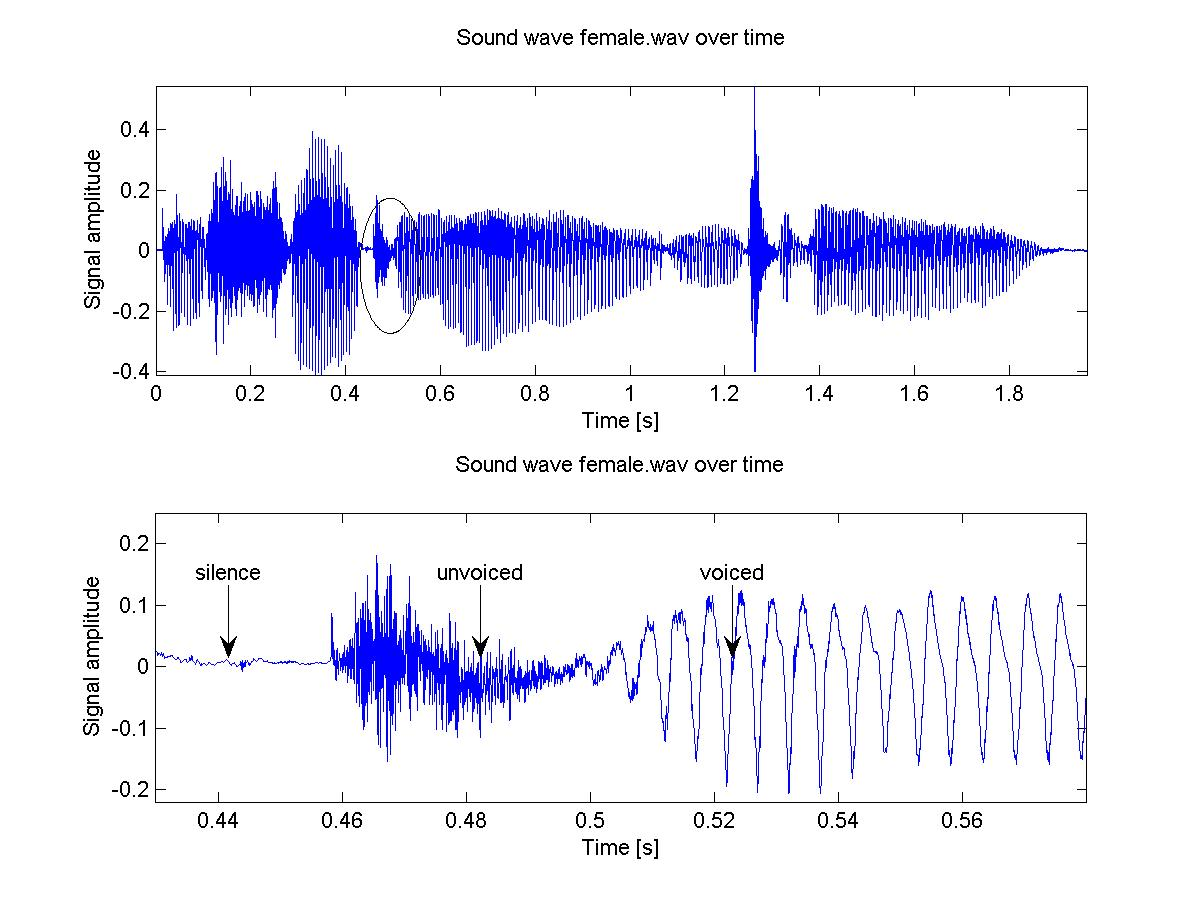
\includegraphics[width=0.85\columnwidth]{figures/2_1.jpg}
			\caption{Female signal voice representation.}
			\label{fig:female_voice}
			\end{figure}

			\begin{figure}[!ht]
			\centering
			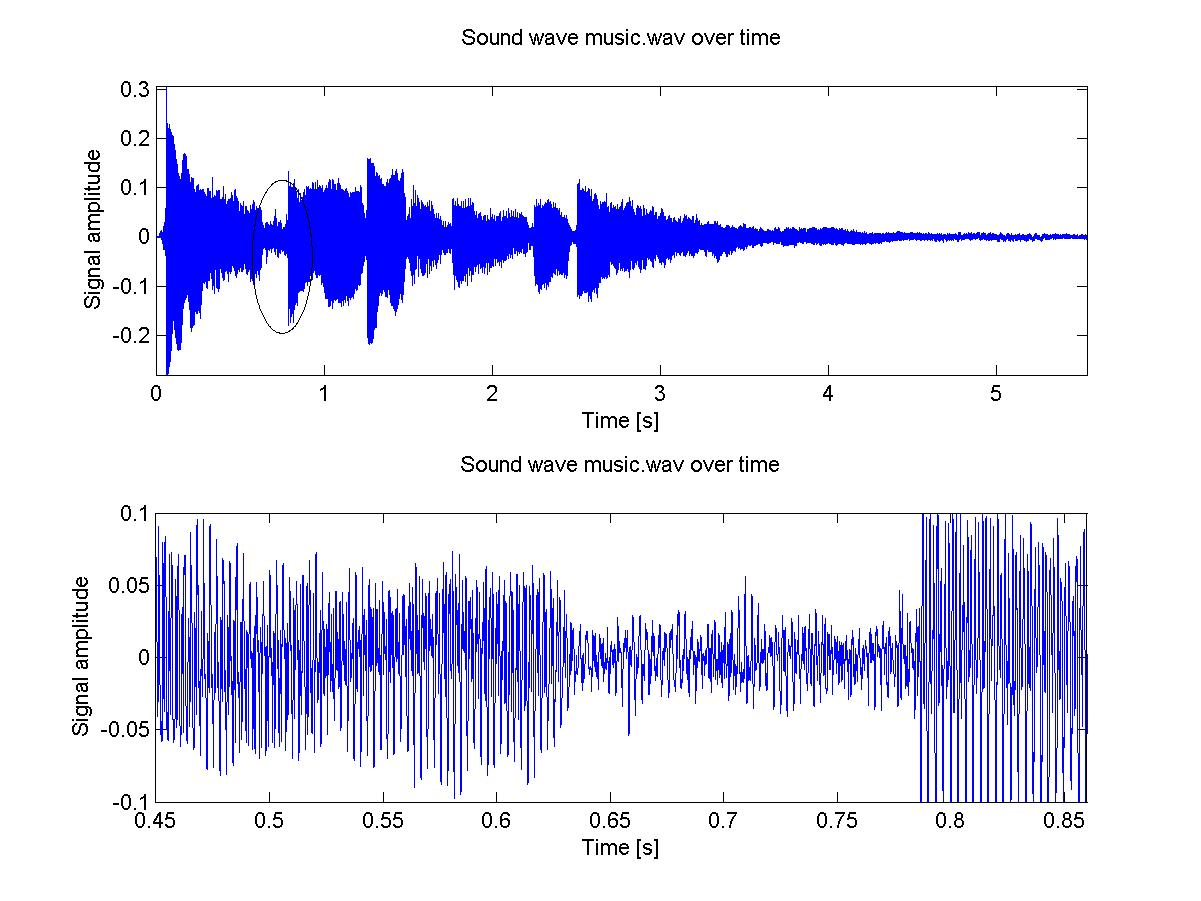
\includegraphics[width=0.85\columnwidth]{figures/2_2.jpg}
			\caption{Augmented section of the female signal representation. Its possible to split in three different regions that
			 represent silence, unvoiced sounds and voiced sound respectively.}
			\label{fig:female_voice_augmented}
			\end{figure}

			\vspace{2mm}
	        		\noindent

			If we want to extract information about frequency we can use the Fourier transform, calculated 
			computationally in a efficient manner using the fast Fourier transform, FFT. The problem with this method 
			is that we lose all time information, and as the hear does, we want a compromise between time and frequency 
			information. For this reason we split the signal in several time intervals, and do the Fourier transform of each. 
			With this method we can obtain the intensity representation for each frequency over time, that is called 	
			spectrogram.

			\vspace{2mm}
	        		\noindent

			The speech, and in our case the female voice consists of voiced and unvoiced sounds. The
			voiced sounds have harmonics and usually corresponds with vowels. Unvoiced sounds have no single determining
			frequency of pattern bus contains a big amount of energy spread over almost all frequencies. Some examples of
			both different regions are marked in Figure~\ref{fig:female_voice_unvoice}].

			\begin{figure}[!ht]
			\centering
			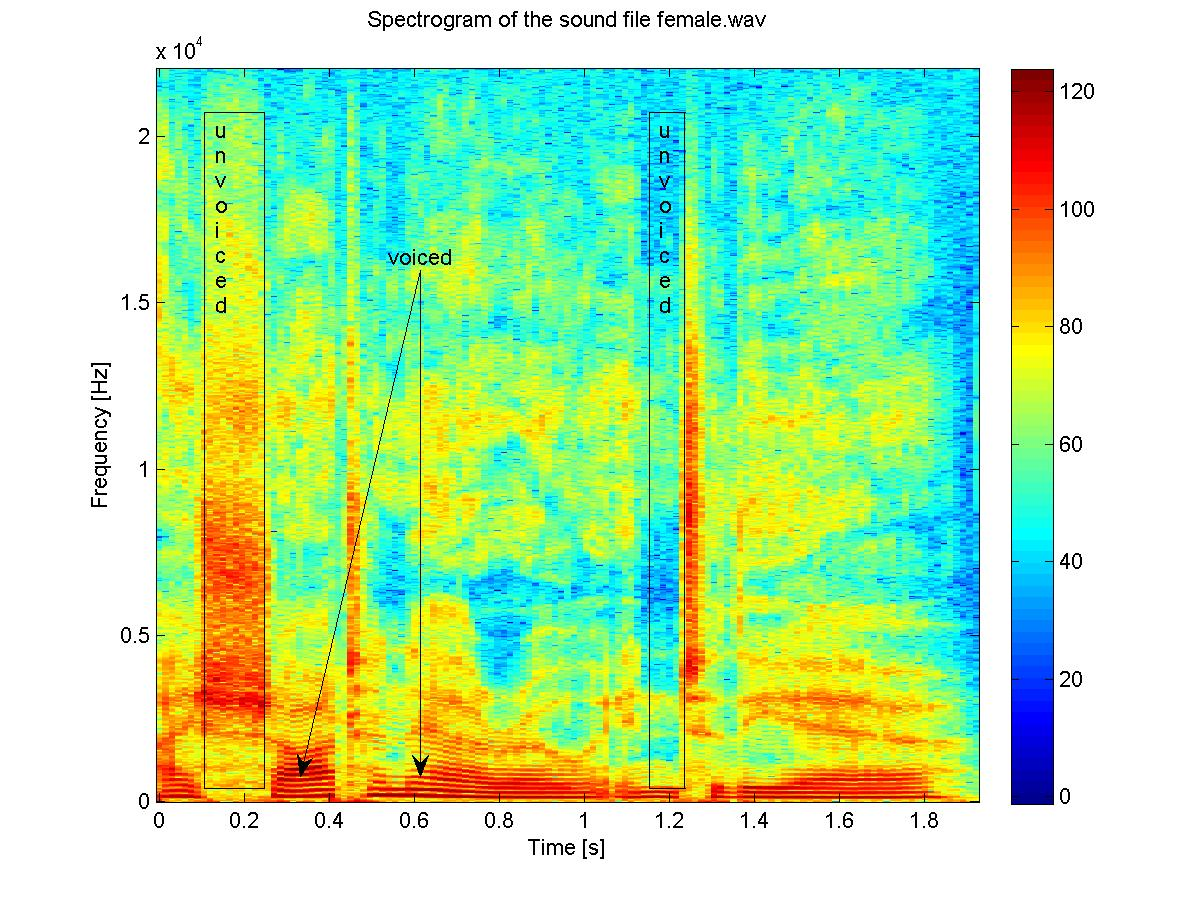
\includegraphics[width=0.85\columnwidth]{figures/2_3.jpg}
			\caption{Voice and unvoice regions for female voice signal.}
			\label{fig:female_voice_unvoice}
			\end{figure}

			The music signal is composed by harmonics. Harmonics are components whose frequency is a multiple of the basic
			frequency f. And they are represented on the spectrograms as bands of signals with high intensity moving up and
			down in unison. Some of there are marked in Figure~\ref{fig:music_harmonics}].

			\begin{figure}[!ht]
			\centering
			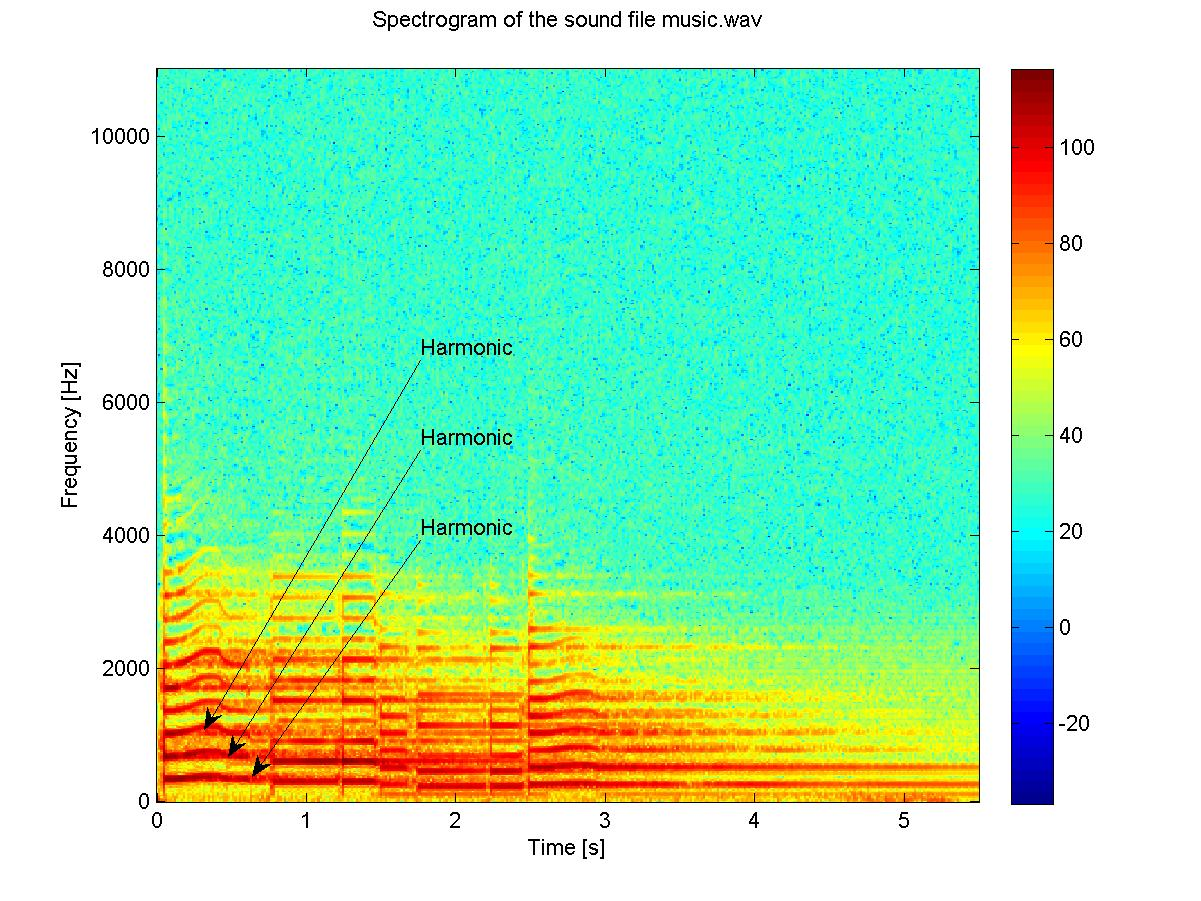
\includegraphics[width=0.85\columnwidth]{figures/2_4.jpg}
			\caption{Harmonics annotation for the music signal spectrogram.}
			\label{fig:music_harmonics}
			\end{figure}

			\vspace{2mm}
	        		\noindent

	\end{itemize}

	\begin{itemize}
		\item	Spectrograms representation gives us a better impression of how sound is perceived, but is not well suited for
			speech recognition. The problem is that still have to much high rate, so another Fourier transform is applied to 
			the data tocalculate the 

			\emph{mel frequency cepstrum coefficients} MFCCs.

	\end{itemize}

\end{itemize}

\begin{itemize}
	\item	After the explanation of both methods and how they works, it may be instructive four our task, speech recognition,
		to make some comparations between female voice and male voice signals, and spectrograms and cepstrograms representations.  

		\begin{itemize}
			\item 	\emph{Which representation do you think is the easiest for you, as a human, to interpret, and why?.}

			\vspace{2mm}
	        		\noindent
			
			Looking at the pictures .....
		\end{itemize}

		\begin{itemize}
			\item  	\emph {Can you see that they represent the same phrase?. Could a computer discover this?. 
				Why/why not?. What about computer?.}

			\vspace{2mm}
	        		\noindent

			Looking at....
		\end{itemize}

		\begin{itemize}
			\item 	\emph {Which matrix, spectral or cepstral, looks the most diagonal to you?}

			\vspace{2mm}
	        		\noindent

			Looking at...
		\end{itemize}
\end{itemize}

\end{document}
